\documentclass[xcolor={svgnames},hyperref={colorlinks,allcolors=Blue}]{beamer}

\usepackage[utf8]{inputenc}
\usetheme{Madrid}
\usecolortheme{beaver}
\setbeamertemplate{theorems}[numbered] 
\usepackage{graphicx}

\usepackage[style=authoryear-comp,backend=biber,natbib,hyperref=true]{biblatex}

\newtheorem{remark}{Remark} %for remark 

\renewcommand\thetheorem{\arabic{lecture}.\arabic{theorem}}
\renewcommand\theremark{\arabic{lecture}.\arabic{remark}}
\makeatletter
\@addtoreset{theorem}{lecture}
\@addtoreset{remark}{lecture}
\makeatother

\usepackage{amsmath}
\usepackage{amssymb}
\usepackage{amsthm}
\usepackage{empheq,mathtools}

\title {Non-Standard Discretization Methods}

\subtitle {for Some Biological Models}

%\author[Arthur, Doe] % (optional, for multiple authors)
%{A.~B.~Arthur\inst{1} \and J.~Doe\inst{2}}

\author{Padmashri Saravanan}

\institute{2018B4PS1039G}

%\institute[VFU] % (optional)
%{
%  \inst{1}%
%  Faculty of Physics\\
%  Very Famous University
%  \and
%  \inst{2}%
%  Faculty of Chemistry\\
%  Very Famous University
%}

\date[10th April 2021] % (optional)
{Mathematical Modelling Project}

\begin{document}

\lecture{Test lecture one}{lone}

\frame{\titlepage}

\begin{frame}
\frametitle{Introduction}
In this project, I will be presenting various numerical schemes that produce differential equations whose dynamics remains unchanged from the underlying continuous equations.\\~\\ They are used to transform the initially continuous problem which has an infinite number of degrees of freedom into a discrete problem where the degree of freedom is inevitably limited.
\end{frame}

\begin{frame}
    \frametitle{Outline}
    \tableofcontents
 \end{frame}
%% To highlight which chapter you're on

\AtBeginSection[]
{
  \begin{frame}
    \frametitle{Table of Contents}
    \tableofcontents[currentsection]
  \end{frame}
}

\section{Stability of Lotka-Volterra Differential Equations}

%% 1st Slide

\begin{frame}
\frametitle{Three types of relationships between two species}
Consider two species X and Y. 
\begin{itemize}
\pause
\item Predator-Prey Model
\begin{itemize}
\item Say X is the prey and Y is the predator.
\pause
\item Presence of X has a positive impact on the growth of Y while the presence of Y has a negative impact on X. 
\end{itemize}

\pause
\item Competition Model
\begin{itemize}
\item X and Y compete for common resources: food, living space, etc.
\end{itemize}

\pause
\item Cooperation Model
\begin{itemize}
\item X and Y positively affect each other's presence. 
\end{itemize}

\end{itemize}
\end{frame}

%% 2nd Slide

\begin{frame}
\frametitle{Modelling the Lotka-Volterra Differential Equations}

\begin{block}{Lotka-Volterra System}
\begin{equation}
	\begin{rcases}
		~\frac{dX}{dt} = X(t)[r_1-a_{1}x(t) - by(t)] \\
		~\frac{dY}{dt} = Y(t)[r_2-cx(t)-a_{2}y(t)] 
	\end{rcases}
	\tag{1}
\end{equation}
\begin{quote}
where $r_1$ and $r_2$ represent the intrinsic growth/decay rate of X and Y, $a_{1}$ and $a_{2}$ are effects caused within the same species, \\ $b$ is the growth effect of X from Y and \\ $c$ is the growth effect of Y from X. 
\end{quote}
\end{block}

\pause
Clearly $a_1 \geqslant$ 0 and $a_2 \geqslant$ 0.
\begin{itemize}
\item Predator-Prey Model
	\begin{itemize}
		\item Presence of X (prey) has a positive impact on the growth of Y (predator) while the presence of Y has a 				negative impact on X.
		\item $b >$ 0, $c >$ 0
	\end{itemize}
\end{itemize}
\end{frame}

\begin{frame}
\frametitle{Modelling the Lotka-Volterra Differential Equations}

\begin{block}{Lotka-Volterra System}
\begin{equation}\label{eq:one}
	\begin{rcases}
		~\frac{dX}{dt} = X(t)[r_1-a_{1}x(t) - by(t)] \\
		~\frac{dY}{dt} = Y(t)[r_2-cx(t)-a_{2}y(t)] 
	\end{rcases}
\end{equation}
\begin{quote}
where $r_1$ and $r_2$ represent the intrinsic growth/decay rate of X and Y, $a_{1}$ and $a_{2}$ are effects caused within the same species, \\ $b$ is the growth effect of X from Y and \\ $c$ is the growth effect of Y from X. 
\end{quote}
\end{block}

Clearly $a_1 \geqslant$ 0 and $a_2 \geqslant$ 0.
\begin{itemize}
\item Competition Model
	\begin{itemize}
		\item X and Y compete for common resources: food, living space, etc.
		\item $b \geqslant$ 0, $c$ $\geqslant$ 0
		\end{itemize}
		
\end{itemize}
\end{frame}

\begin{frame}

\frametitle{Modelling the Lotka-Volterra Differential Equations}

\begin{block}{Lotka-Volterra System}
\begin{equation} 
	\begin{rcases}
		~\frac{dX}{dt} = X(t)[r_1-a_{1}x(t) - by(t)] \\
		~\frac{dY}{dt} = Y(t)[r_2-cx(t)-a_{2}y(t)] 
	\end{rcases}
	\tag{1}
\end{equation}
\begin{quote}
where $r_1$ and $r_2$ represent the intrinsic growth/decay rate of X and Y, $a_{1}$ and $a_{2}$ are effects caused within the same species, \\ $b$ is the growth effect of X from Y and \\ $c$ is the growth effect of Y from X. 
\end{quote}
\end{block}

Clearly $a_1 \geqslant$ 0 and $a_2 \geqslant$ 0.
\begin{itemize}
\item Cooperation Model
	\begin{itemize}
		\item X and Y positively affect each other's presence. 
		\item $b \leqslant$ 0, $c \leqslant$ 0
	\end{itemize}

\end{itemize}
\end{frame}

\begin{frame}
\frametitle{Stability Analysis for the Lotka-Volterra Model}
For System $(1)$ to possess a equilibrium point $(X^*,Y^*)$, it must satisfy: 
\\
\begin{equation}
	a_1X^* + bY^* - r_1 = 0
\end{equation}
and 
\begin{equation}
	cX^* + a_2Y^* - r_2 = 0
\end{equation}
\pause
Solving equations (2) and (3) for $X^* $ and $Y^*$, we get:
\begin{equation}
	~X^* = \frac{r_1a_2-r_2b}{a_1a_2-bc}~,Y^* = \frac{r_2a_1-r_1c}{a_1a_2-bc}~
\end{equation}
	
\end{frame}

\begin{frame}
\frametitle{Stability Analysis for the Lotka-Volterra Model}

\begin{block}{Classification of an Equilibrium Point}
The equilibrium point ($X^*$,$Y^*$) is said to be \textbf{stable} if for any open neighbourhood U of ($X^*,Y^*$) $\exists$ an open neighbourhood V of ($X^*,Y^*$) such that if ($X_0,Y_0$) $\in$ V, then (X(t,$X_0$),Y(t,$Y_0$)) $\in$ U $\forall$ t $\geqslant$ 0. \\~\\ 

If ($X^*$,$Y^*$) is stable and $\lim_{t\to\infty}$ (X(t,$X_0$),Y(t,$Y_0$)) = ($X^*$,$Y^*$) $\forall$ ($X_0,Y_0$) in an open neighbourhood W of ($X^*$,$Y^*$), then ($X^*$,$Y^*$) is \textbf{asymptotically stable}. \\~\\

If W $=$ $\mathbb{R}^2$, then ($X^*$,$Y^*$) is \textbf{globally asymptotically stable}.
\end{block}

\pause
Stability means that the solution of the differential equation will not leave the $\epsilon$-ball, \pause but asymptotic stability means that the solution does not leave the $\epsilon$-ball and goes to the equilibrium point.
	\end{frame}

%\begin{frame}
%\frametitle{Stability Analysis for the Lotka-Volterra Model}
%
%	\begin{theorem}
%	If System (1) has an asymptotically stable positive equilbrium point $(X^*,Y^*)$, then $(X^*,Y^*)$ is a globally asymptotically stable point if $a_1 > 0$ and $a_2 > 0$.
%	\end{theorem}
%
%%\pause
%%Decreasing $\epsilon$ will force the initial condition to approach the zero in the stable case and not the solution at infinity.
%	
%\end{frame}


\AtBeginSection[]
{
  \begin{frame}
    \frametitle{Table of Contents}
    \tableofcontents[currentsection]
  \end{frame}
}

\section{Classical Discretization}


\begin{frame}
\frametitle{Forward Euler Method}
\framesubtitle{Numerical Schemes}

Using Taylor series expansion and neglecting higher order terms, \pause \\ we arrive at: \\
	\begin{equation}
		\frac{dX}{dt} = \frac{X(t+h)-X(t)}{h} ~and~
		\frac{dY}{dt} = \frac{Y(t+h)-Y(t)}{h}
	\end{equation}
	\\~\\ where h is the step size of the Euler method. \\~\\
	\pause
	This results in the Forward Euler Method having a \textit{local truncation error} of O($h^2$), and therefore is a first order technique. 
	
\end{frame}

\begin{frame}
\frametitle{Forward Euler Method}
\framesubtitle{Numerical Schemes}

Replacing System (1) with Equations (5), and taking n = $\frac{t}{h}$, $X(t) = X(nh) =  X(n)$, and $Y(t) = Y(nh) = Y(n)$, we arrive at the difference system:

\pause
\begin{block}{Difference System for Lotka-Volterra Model}
	\begin{equation}
		\begin{rcases}
		~X(n+1) = X(n)[1+r_1h-a_1hX(n)-bhY(n)] \\ 
		~Y(n+1) = Y(n)[1+r_2h-chX(n)-a_2hY(n)[
		\end{rcases}
	\end{equation}
\end{block}

\end{frame}

\begin{frame}
\frametitle{Plotting the Lotka-Volterra System}
\framesubtitle{Predator-Prey Model}
We implement the Forward Euler Method on MATLAB and compare the Phase Portraits with various parameter modifications: ($a_1 >$ 0, $a_2 >$ 0) \\ 
\begin{itemize}
\pause
\item \textbf{Case I:} Increasing Parameters
	\begin{center}
		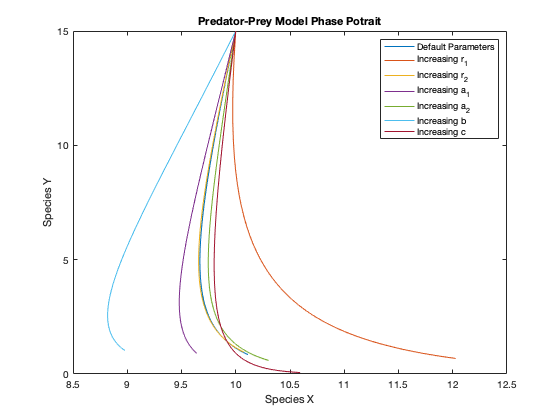
\includegraphics[width = 0.7\textwidth]{increasing_LV.png}
	\end{center}

\end{itemize}
\end{frame}


\begin{frame}
\frametitle{Plotting the Lotka-Volterra System}
\framesubtitle{Predator-Prey Model}
We implement the Forward Euler Method on MATLAB and compare the Phase Portraits with various parameter modifications: ($a_1 >$ 0, $a_2 >$ 0) \\ 
\begin{itemize}
\item \textbf{Case II:} Decreasing Parameters
	\begin{center}
		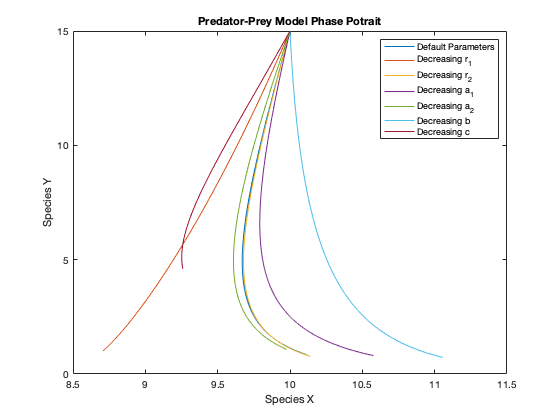
\includegraphics[width = 0.7\textwidth]{decreasing_LV.png}
	\end{center}

\end{itemize}
\end{frame}

\begin{frame}
\frametitle{Plotting the Lotka-Volterra System}
\framesubtitle{Predator-Prey Model}
We implement the Forward Euler Method on MATLAB and compare the Phase Portraits with various parameter modifications: ($a_1 >$ 0, $a_2 >$ 0) \\ 
\begin{itemize}
\item \textbf{Case III:} Altering Initial Conditions: X0
	\begin{center}
		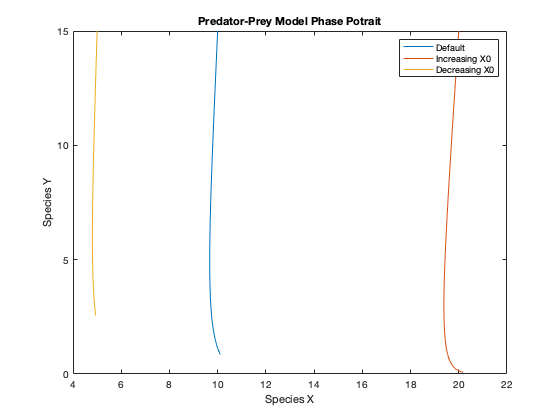
\includegraphics[width = 0.7\textwidth]{1.png}
	\end{center}

\end{itemize}
\end{frame}

\begin{frame}
\frametitle{Plotting the Lotka-Volterra System}
\framesubtitle{Predator-Prey Model}
We implement the Forward Euler Method on MATLAB and compare the Phase Portraits with various parameter modifications:($a_1 >$ 0, $a_2 >$ 0) \\ 
\begin{itemize}
\item \textbf{Case IV:} Altering Initial Conditions: Y0
	\begin{center}
		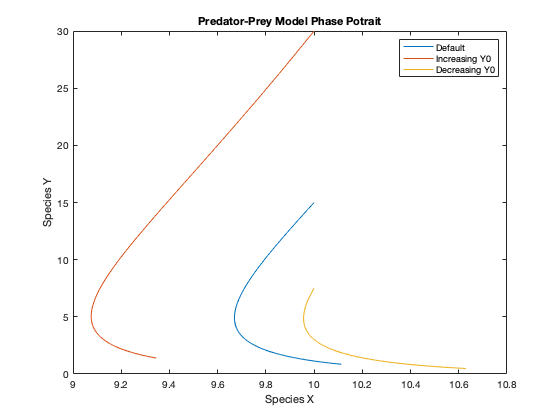
\includegraphics[width = 0.7\textwidth]{alteringY0.png}
	\end{center}

\end{itemize}
\end{frame}

\begin{frame}
\frametitle{Plotting the Lotka-Volterra System}
\framesubtitle{Predator-Prey Model}
In all 4 cases, we see that the equilibrium point remains asymptotically stable, regardless of the modifications that are made, when $a_1 >$ 0, $a_2 >$ 0. \\~\\ Now, we plot and compare the phase portraits for Systems (1) and  (6) when $a_1 <$ 0, $a_2 <$ 0.
\end{frame}

\begin{frame}
\frametitle{Plotting the Lotka-Volterra System}
\framesubtitle{Predator-Prey Model}
Phase Portrait of System $(1)$ when $a_1 <$ 0, $a_2 <$ 0: 
	\begin{center}
		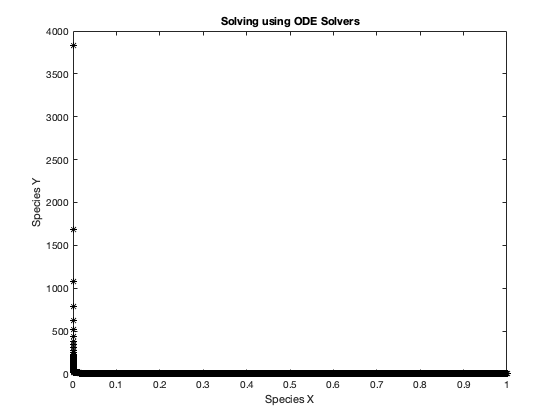
\includegraphics[width = 0.8\textwidth]{ode45.png}
	\end{center}

\end{frame}

\begin{frame}
\frametitle{Plotting the Lotka-Volterra System}
\framesubtitle{Predator-Prey Model}
Phase Portrait of System $(6)$ when $a_1 <$ 0, $a_2 <$ 0: 
	\begin{center}
		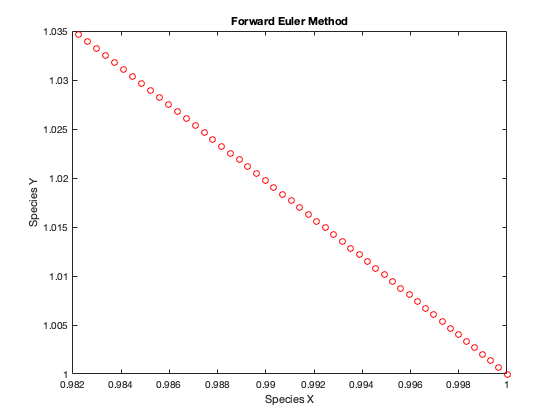
\includegraphics[width = 0.8\textwidth]{fwdeuler.png}
	\end{center}
\end{frame}

\begin{frame}
\frametitle{Limitations of Forward Euler Method}
\framesubtitle{Alternative Numerical Schemes}
As seen in the above slides, the dynamics of System (6) is different from that of System (1) and can cause chaotic behaviour. (Ushiki, 1982) \\~\\ 
\pause
An alternative well-known method is to let System (1) have piecewise constant arguments:
\begin{equation} 
	\begin{rcases}
		~\frac{dX}{dt} = X(t)[r_1-a_{1}x(\lfloor t \rfloor) - by(\lfloor t \rfloor)] \\
		~\frac{dY}{dt} = Y(t)[r_2-cx(\lfloor t \rfloor)-a_{2}y(\lfloor t \rfloor)] 
	\end{rcases}
\end{equation}

where 0 $\leqslant n \leqslant t <$ n + 1, and $\lfloor t \rfloor$ is the greatest integer in t. 

\end{frame}

%\begin{frame}
%\frametitle{Limitations of Forward Euler Method}
%\framesubtitle{Alternative Numerical Schemes}
%Integrating both sides of System (7) gives us: 
%\begin{equation}
%	\begin{rcases}
%	~X(t) = X(n)exp[r_1-a_1X(n)-bY(n)],\\
%	~Y(t) = Y(n)exp[r_2-cX(n)-a_2Y(n)]
%	\end{rcases}
%\end{equation}
%	\begin{center}
% 		t $\in$ [n,n+1)
%	\end{center}
%
%\pause
%~\\ Letting t $\rightarrow$ n+1, we arrive at the following difference equations:
%\begin{equation}
%	\begin{rcases}
%	~X(n+1) = X(n)exp[r_1-a_1X(n)-bY(n)],\\
%	~Y(n+1) = Y(n)exp[r_2-cX(n)-a_2Y(n)]
%	\end{rcases}
%\end{equation}
%\end{frame}

%\begin{frame} 
%\frametitle{Implementing Piecewise Constant Method on the Lotka-Volterra Model}
%\framesubtitle{Alternative Numerical Schemes}
%\begin{itemize}
%\pause
%\item \textbf{Case I:} Predator-Prey Model
%	\begin{center}
%		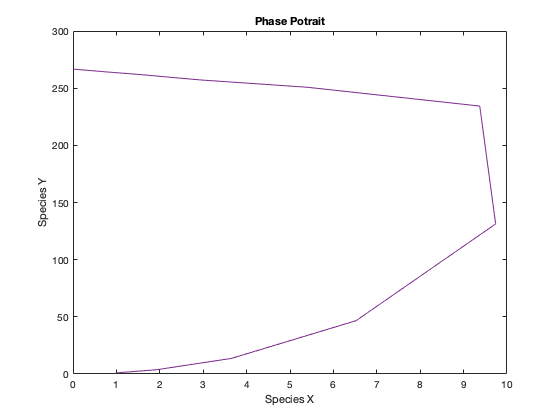
\includegraphics[width = 0.75\textwidth]{predprey.png}
%	\end{center}
%\end{itemize}
%\end{frame}
%
%\begin{frame} 
%\frametitle{Implementing Piecewise Constant Method on the Lotka-Volterra Model}
%\framesubtitle{Alternative Numerical Schemes}
%\begin{itemize}
%\item \textbf{Case II:} Competition Model
%	\begin{center}
%		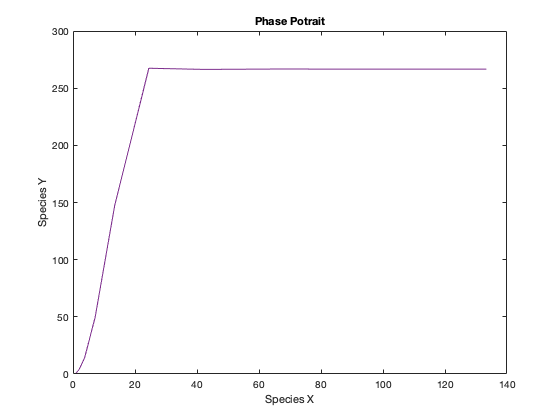
\includegraphics[width = 0.75\textwidth]{competition.png}
%	\end{center}
%\end{itemize}
%\end{frame}
%
%\begin{frame} 
%\frametitle{Implementing Piecewise Constant Method on the Lotka-Volterra Model}
%\framesubtitle{Alternative Numerical Schemes}
%\begin{itemize}
%\item \textbf{Case III:} Cooperation Model
%	\begin{center}
%		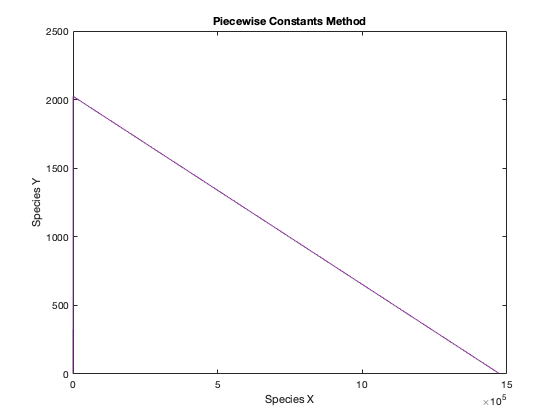
\includegraphics[width = 0.75\textwidth]{cooperation.png}
%	\end{center}
%\end{itemize}
%\end{frame}
%
%\begin{frame}
%\frametitle{Dynamical Behaviour of System (9)}
%As investigated by Krawcewicz and Rogers (1990) for the Cooperation Model, and by Jian and Rogers (1987) for the Competition Model, it was seen that System (9) displayed a rather different dynamical behavior from its continuous System (1). 
%\end{frame}

\AtBeginSection[]
{
  \begin{frame}
    \frametitle{Table of Contents}
    \tableofcontents[currentsection]
  \end{frame}
}

\section{Leslie Predator-prey Model}

\begin{frame} 
\frametitle{Leslie Predator-prey Model}

Predator's response function is assumed to be logistic, but its carrying capacity is a function of the prey density. 

\pause	
	\begin{equation}
		\begin{rcases}
		~\frac{dx}{dt} = x(t)[\gamma_1 - a_1x(t) - by(t)] \\
		~\frac{dy}{dt} = y(t)[\gamma_2 - a_2\frac{y(t)}{x(t)}]
		\end{rcases}
	\end{equation}

	\begin{quote}
	where all the parameters $\gamma_1, a_1, b,\gamma_2, a_2$ are positive real numbers. 
	\end{quote}
	
\pause
System (8) has a unique positive equilbrium point $(x^*,y^*)$ with 
	\begin{equation} 
	~x^* = \frac{\gamma_1a_2}{a_1a_2+b\gamma_2}, y^* = \frac{\gamma_1\gamma_2}{a_1a_2+b\gamma_2}
	\end{equation}
\pause
The equilibrium point $(x^*,y^*)$ is asymptotically stable $\forall$ parameters $>$ 0.
\end{frame}

\begin{frame} 
\frametitle{Implementing The Leslie Model}
When implementing system (8) on MATLAB and plotting the solution profiles and phase portrait: 

	\begin{center}
	\pause
		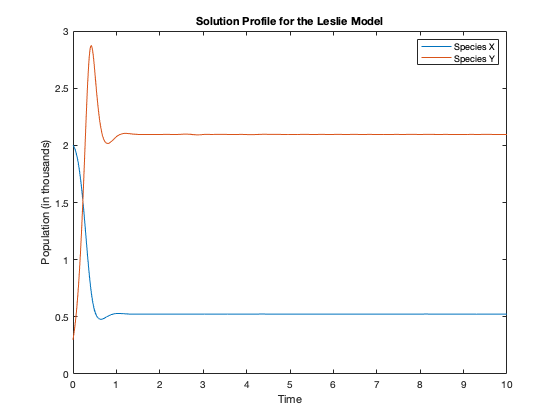
\includegraphics[width = 0.75\textwidth]{leslie1.png}
	\end{center}

\end{frame}

\begin{frame} 
\frametitle{Implementing The Leslie Model}
When implementing system (10) on MATLAB and plotting the solution profiles and phase portrait: 

	\begin{center}
		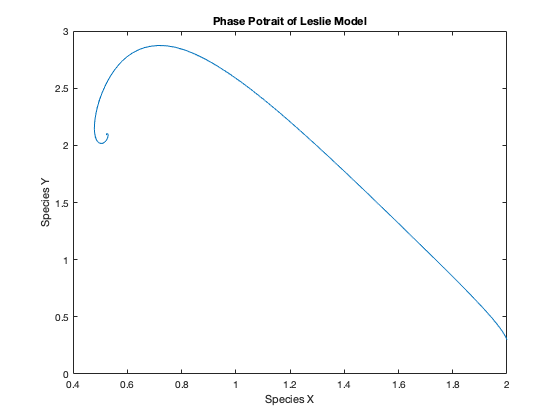
\includegraphics[width = 0.75\textwidth]{leslie2.png}
	\end{center}

\end{frame}

\begin{frame}
\frametitle{Schur-Cohn Criterion for Asymptotic Stability}

\begin{block} {Definition}
The \textit{trace} of a n x n matrix A (tr A) is the sum of its diagonal elements.
\end{block}

\pause
The \textbf{Schur-Cohn criterion} must be satisfied for local asymptotic stability, and it is satisfied when the eigenvalues $\lambda_i$ of the Jacobian matrix are such that $|\lambda_i| <$ 0.

\pause
\begin{theorem}
For $|\lambda_i| <$ 0, it is necessary and sufficient that for the Jacobian matrix J,
   % \begin{center}
    	\begin{center}
	$|tr ~J| < 1 + det ~J < 2$
	\end{center}
where det J is the determinant of J.
    %\end{center}
\end{theorem}

\end{frame}

\begin{frame}
\frametitle{Conditions of Schur-Cohn Criterion}
We can split the 2 inequalities of Theorem 1.2 into 3 different conditions:
\pause
\begin{enumerate}
	\item det J $<$ 1 \pause
	\item 1 - tr J + det J $>$ 0 \pause
	\item 1 + tr J + det J $>$ 0
\end{enumerate}

\end{frame}

\begin{frame}
\frametitle{Discretizing the Leslie Predator-prey Model}

We propose the discrete model:

	\begin{equation}
		\begin{rcases}
		~\frac{x(t+h)-x(t)}{\varphi_1(h)} = \gamma_1x(t) - a_1x(t)x(t+h)-bx(t+h)y(t) \\
		~\frac{y(t+h)-y(t)}{\varphi_2(h)} = \gamma_2y(t) - \frac{a_2y(t)y(t+h)}{x(t)}
		\end{rcases}
	\end{equation}

\pause
which gives us the difference system:
	
	\begin{equation}
		\begin{rcases}
		~x(n+1) = \frac{x(n)(1+\gamma_1\varphi_1(h))}{1+a_1\varphi(h)x(n)+b\varphi_1(h)y(n)} = F(x(n),y(n)) \\
		~y(n+1) = \frac{x(n)y(n)(1+\gamma_2\varphi_2(h))}{x(n)+a_2\varphi_2(h)y(n)} = G(x(n),y(n))
		\end{rcases}
	\end{equation}

\end{frame}

\begin{frame}
\frametitle{Linearizing the Leslie Model}

Linearizing system (11) around $(x^*,y^*)$ gives us the coefficient matrix: 

\begin{center}
\pause
    B = $\begin{pmatrix}
    1 - \frac{a_1\varphi_1(h)x^*}{1+\gamma_1\varphi_1(h)} & -\frac{b\varphi_1(h)x^*}{1+\gamma_1\varphi_1(h)} \\~\\
    \frac{a_2\varphi_2(h)y^*^2}{x^*(x^*+a_2\varphi_2(h)y^*} & \frac{x^*}{x^* + a_2\varphi_2(h)y^*}
    \end{pmatrix}$

\end{center}

\pause
Through direct checking, we see that all 3 Schur-Cohn conditions are satisfied and hence, $(x^*,y^*)$ is asymptotically stable.
\end{frame}

\begin{frame}
\frametitle{Limitations of the Leslie Model}
%Some terminologies before we look at the model: \pause
	\begin{itemize}
	
	\item \textbf{Proliferation} is a rapid increase in population density, and will often create an overpopulation problem. 		\pause
	\item This causes an environmental imbalance, and is not considered in the Leslie Model. \pause
	\item This model also does not take into consideration the \textbf{Allee Effect} \pause
	\item An Allee Effect is a positive correlation between individual fitness and population size over some finite time interval (like mate limitation). 
	\end{itemize}


\end{frame}


\begin{frame}
\frametitle{Limitations of the Leslie Model}
	\begin{itemize}
	\item The Allee Effect significantly changes the dynamics of the original system. \pause
	\item The model used above also does not consider non-topological equivalent behaviours.  \pause 
	\item For instance, species that are endangered species have a low probability of locating responsive mates or a 			biased sex-ratio. 
	\end{itemize}
	
\end{frame}

\begin{frame}
\frametitle{Recommendations for the Leslie Model}

With a strong Allee effect on prey, zero, one or two equilibrium points can exist. (González-Olivares, Mena-			Lorca, Rojas-Palma and Flores, 2007). \pause \\~\\ 
To factor in the limitations previously mentioned, the Leslie-Grower Model is a more apt model, in which the Allee threshold is a parameter in the system. 

\end{frame}


\AtBeginSection[]
{
  \begin{frame}
    \frametitle{Table of Contents}
    \tableofcontents[currentsection]
  \end{frame}
}

\section{Other Nonstandard Numerical Schemes}

\begin{frame}
\frametitle{Simple Predator-Prey Model}
We consider the model:
\pause
	\begin{equation}
		\begin{rcases}
		~\frac{dx}{dt} = \alpha x +\beta xy~\\
		~\frac{dy}{dt} = \gamma y + \delta xy~
		\end{rcases}
	\end{equation}
	
	\begin{quote}
	where x(t): density of the prey at time t, and \\ y(t): density of predator at time t. 
	\end{quote}

\pause	
If \begin{equation} \alpha < 0, \beta >0, \gamma > 0, \delta < 0 \end{equation} then $(-\alpha/\beta, -\gamma/\delta)$ is the only positive equilibrium point of system (12).

\end{frame}

\begin{frame}
\frametitle{Implementing the Simple Predator-Prey Model in MATLAB}

Taking $\alpha = -1, \beta = 0.01, \gamma = 0.5 ~and~ \delta = -0.01,$ we plot the solution profile and phase portrait for System (12). Using these parameters, the only positive equilibrium point is (100,50). 

	\begin{center}
	\pause
		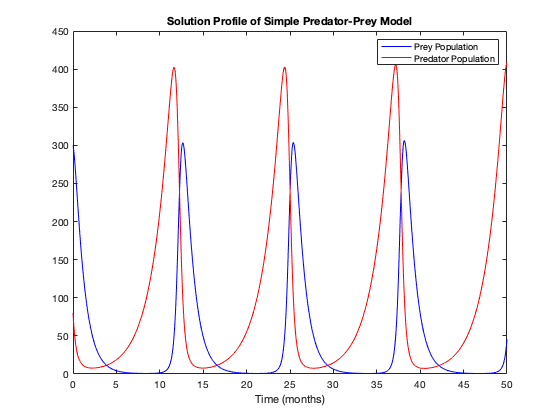
\includegraphics[width = 0.7\textwidth]{simple1.png}
	\end{center}

\end{frame}

\begin{frame}
\frametitle{Implementing the Simple Predator-Prey Model in MATLAB}

Taking $\alpha = -1, \beta = 0.01, \gamma = 0.5 ~and~ \delta = -0.01,$ we plot the solution profile and phase portrait for System (12). Using these parameters, the only positive equilibrium point is (100,50).

	\begin{center}
	\pause
		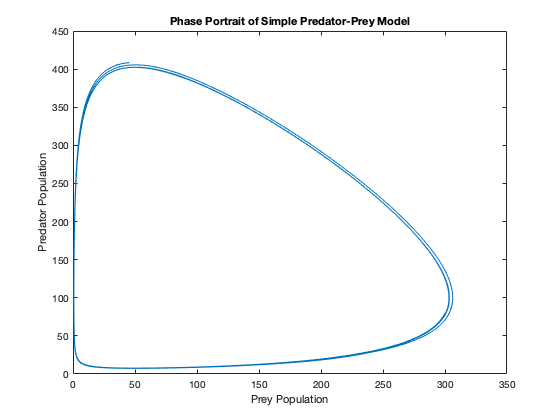
\includegraphics[width = 0.7\textwidth]{simple2.png}
	\end{center}

\end{frame}

\begin{frame}
\frametitle{Discretizing the Simple Predator-Prey Model}
Recall: \\~\\
\pause
The Forward Euler method replaces the derivative $\frac{dy}{dt}$ with $\frac{y(t+h)-y(t)}{h}$, where \textit{h} is the step size. \\~\\ 
\pause
In the Mickens discretization scheme, this is taken one step further and the derivative is replaced with $\frac{y(t+h)-y(t)}{\phi(h)}$, \pause where $\phi(h)$ is a continuous function of step size \textit{h}, and is such that\\ 
\begin{center}
$\phi(h)$ = h + O(h), 0 $<$ $\phi(h)$ $<$ 1, h $\rightarrow$ 0
\end{center}
\pause If the Mickens discretization scheme is applied to the system (12), the solution either spirals in towards $(x^*,y^*)$ or spirals out of the equilibrium point $(x^*,y^*)$. 
\end{frame}

\begin{frame}
\frametitle{Implementing the Discretized Simple Predator-Prey Model in MATLAB}

	\begin{center}
		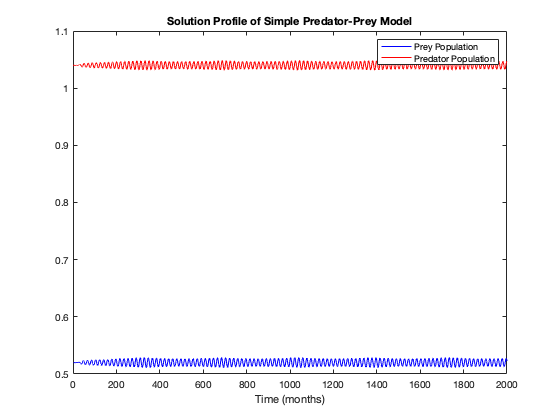
\includegraphics[width = 0.85\textwidth]{mickens1.png}
	\end{center}

\end{frame}

\begin{frame}
\frametitle{Implementing the Discretized Simple Predator-Prey Model in MATLAB}

	\begin{center}
		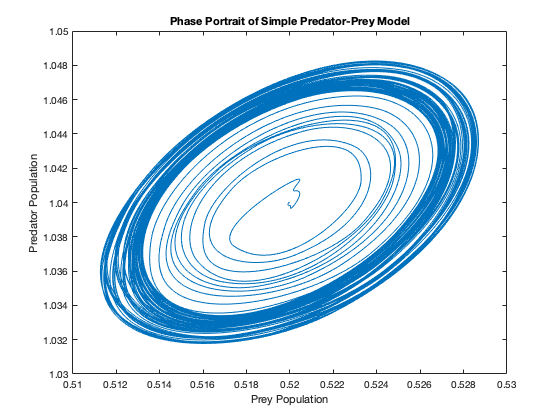
\includegraphics[width = 0.85\textwidth]{mickens2.png}
	\end{center}

\end{frame}



\AtBeginSection[]
{
  \begin{frame}
    \frametitle{Table of Contents}
    \tableofcontents[currentsection]
  \end{frame}
}

\section{Kolmogorov Model of Cooperative Systems}

\begin{frame}
\frametitle{Cooperative Systems}
\framesubtitle{Robert May's Model}

Consider two species with population densities x(t) and y(t). \pause

	\begin{equation}
		\begin{rcases}
		~\frac{dx}{dt} = r_1x(t)(1-\frac{x(t)}{\beta_1+ \alpha_1y(t)} )\\
		~\frac{dy}{dt} = r_2y(t)(1-\frac{y(t)}{\beta_2+\alpha_2x(t)})
		\end{rcases}
	\end{equation}
	where $r_1$,$r_2$, $\alpha_1$, $\alpha_2$, $\beta_1$, $\beta_2$ are positive numbers. 

\pause
If $\alpha_1\alpha_2 <$ 1, then $\exists$ a positive equilibrium point $(x^*,y^*)$ which satisfies the equations: 
	\begin{equation}
		\begin{rcases}
		-x^* + \alpha_1y^* = -\beta_1 \\
		\alpha_2x^* - y^* = -\beta_2
		\end{rcases}
	\end{equation}

\end{frame}

\begin{frame}
\frametitle{Stability of Robert May's Model}
The linearized system around $(x^*,y^*)$ has the coefficient matrix: 

\begin{center}
B = $\begin{pmatrix}
    e^{-r_1} & \alpha_1(1-e^{-r_1}) \\~\\
    ~\alpha_2(1-e^{-r_2}) & e^{-r_2}
    \end{pmatrix}$
\end{center}

\pause
Through direct checking, we can see that matrix B satisfies the Schur-Cohn criterion and therefore, makes $(x^*,y^*)$  a locally asymptotically stable equilibrium point.

\end{frame}

\begin{frame}
\frametitle{Implementing the Robert May Model in MATLAB}

	\begin{center}
		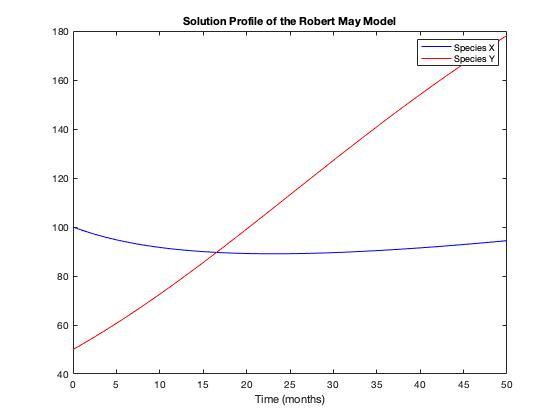
\includegraphics[width = 0.85\textwidth]{robert.png}
	\end{center}

\end{frame}

\begin{frame}
\frametitle{Implementing the Robert May Model in MATLAB}

	\begin{center}
		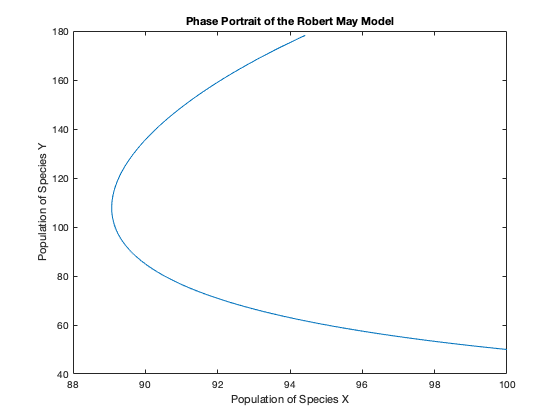
\includegraphics[width = 0.85\textwidth]{robert2.png}
	\end{center}

\end{frame}

\AtBeginSection[]
{
  \begin{frame}
    \frametitle{Table of Contents}
    \tableofcontents[currentsection]
  \end{frame}
}

\section{Conclusion}

\begin{frame}
\frametitle{Concluding Statements}

We have gone through and implemented the various non-standard discretization Lotka-Volterra models, classical discretization, the Leslie model, further numerical schemes and finally a Kolmogorov Model of cooperative systems, and discussed its local stability. 

\pause
~\\ Apart from the recommendations and limitations mentioned in my presentation, there is definitely more scope to make biological models that factor in more aspects of the environment of the species, making it more precise and reliable.

\end{frame}

\AtBeginSection[]
{
  \begin{frame}
    \frametitle{Table of Contents}
    \tableofcontents[currentsection]
  \end{frame}
}

\section{References}

\begin{thebibliography}{10}

\bibitem{Ushiki1982}[Ushiki, 1982]
S. Ushiki.
\newblock Central Difference Schemes and Chaos,
\newblock \emph{ Physics D, 4, 407-424}, 1982.

\bibitem{KrawRogers}[Krawcewicz and Rogers, 1990]
W. Krawcewicz and T.D. Rogers.
\newblock Perfect harmony: the discrete dynamics of cooperation,
\newblock \emph{J. Math. Biol. 28, 383-410}, 1990

\bibitem{JianRogers}[Jian and Rogers, 1987]
H. Jian and T.D. Rogers.
\newblock The discrete dynamics of symmetric competition in the plane,
\newblock \emph{J. Math. Biol. 25, 573-596}, 1987

\bibitem{Moghadasetal}[Moghadas, Alexander, Corbett, Gumel, 2003]
S. Moghadas, M. Alexander, B. Corbett and A. Gumel
\newblock A Positivity-preserving Mickens-type Discretization of an Epidemic Model
\newblock \emph{Journal of Difference Equations and Applications, 9}, 2003

\bibitem{Berecetal}[L. Berec, E. Angulo and F. Courchamp]
L. Berec, E. Angulo and F. Courchamp
\newblock Multiple Allee effects and population management
\newblock \emph{Trends Ecol. Evol., 22, 185-191}, 2007

\bibitem{Shabbiretal}[Shabbir, M.S., Din, Q., Safeer, M. et al.]
Shabbir, M.S., Din, Q., Safeer, M. et al.
\newblock A dynamically consistent nonstandard finite difference scheme for a predator–prey model. 
\newblock \emph{Advanced Differential Equations, 381}, 2019

\end{thebibliography}

\begin{frame}

\begin{center}
Thank you!
\end{center}

\end{frame}

%\AtBeginSection[]
%{
%  \begin{frame}
%    \frametitle{Table of Contents}
%    \tableofcontents[currentsection]
%  \end{frame}
%}
%
%\section{Citation}
%
%\begin{block}{Open Questions}
%Is every even number the sum of two primes?
%\cite{Goldbach1742}
%\end{block}


\end{document}
    